% !TEX root = ../main.tex

% Indicate the main file. Must go at the beginning of the file.

%--------------------------------------------------------------------------------
% CHAPTER Results
%--------------------------------------------------------------------------------


\chapter{Prototyp Sniffer} % Protoypen Test Main chapter title -> Sniffer Prototyp!?
\label{Prototyp Sniffer} % Change X to a consecutive number; for referencing this chapter elsewhere, use \ref{ChapterX}

%---------------------------------------------------------------------------------
% SECTION 1
%---------------------------------------------------------------------------------

\section{FPGA}
\label{sec:ResultatFPGA}
Der Test zur Datenauswertung im FPGA wurde, wie in Kapitel
\ref{sub:FPGADecSPITest} beschrieben, durchgeführt. Mittels der Software "'Picoscope 7"' konnten die ausgegebenen Daten \textit{MOSI} mit dem dazugehörigen \textit{SCLK} und dem Chipselect \textit{CS} gleich als SPI interpretiert und entschlüsselt dargestellt werden.
Im Verlaufe der Arbeit wurde das FPGA und dessen Decodierung in zwei Szenarien getestet.
Das eine Szenario ist der Test ohne die Zusatzimplementierung eines Puffers und somit das direkte Schreiben auf die SPI sobald ein Nutzdatenbyte ausgewertet wurde.
Im zweiten Szenario wurde ein 64 Bit grosser Puffer vor der SPI implementiert, um die Zeit zwischen der Datenübertragung auf der SPI zu verlängern.
In den folgenden Unterkapiteln werden die Resultate beider Szenarien aufgezeigt.

\subsection{Test ohne 64-Bit-Puffer Implementierung}
\label{sub:ResultatFPGAnoBuff}
Bei diesem Testszenario war kein Unterschied, ob das Signal alle 1 ms oder alle 100 ms übertragen wurde, feststellbar. In beiden Fällen werden mit
der Software \textit{Picoscope 7} die gleichen Übertragungsdaten angezeigt und somit die gleichen Werte entschlüsselt dargestellt.

In Abbildung \ref{fig:ResultatFPGANoBuff} ist dass vom Picoscope eingelesene SPI Signal mit MOSI, SCLK und CS zu sehen. Bei dieser Übertragung handelt es sich um ein Master-Frame.


\begin{figure}[H]
    \centering
    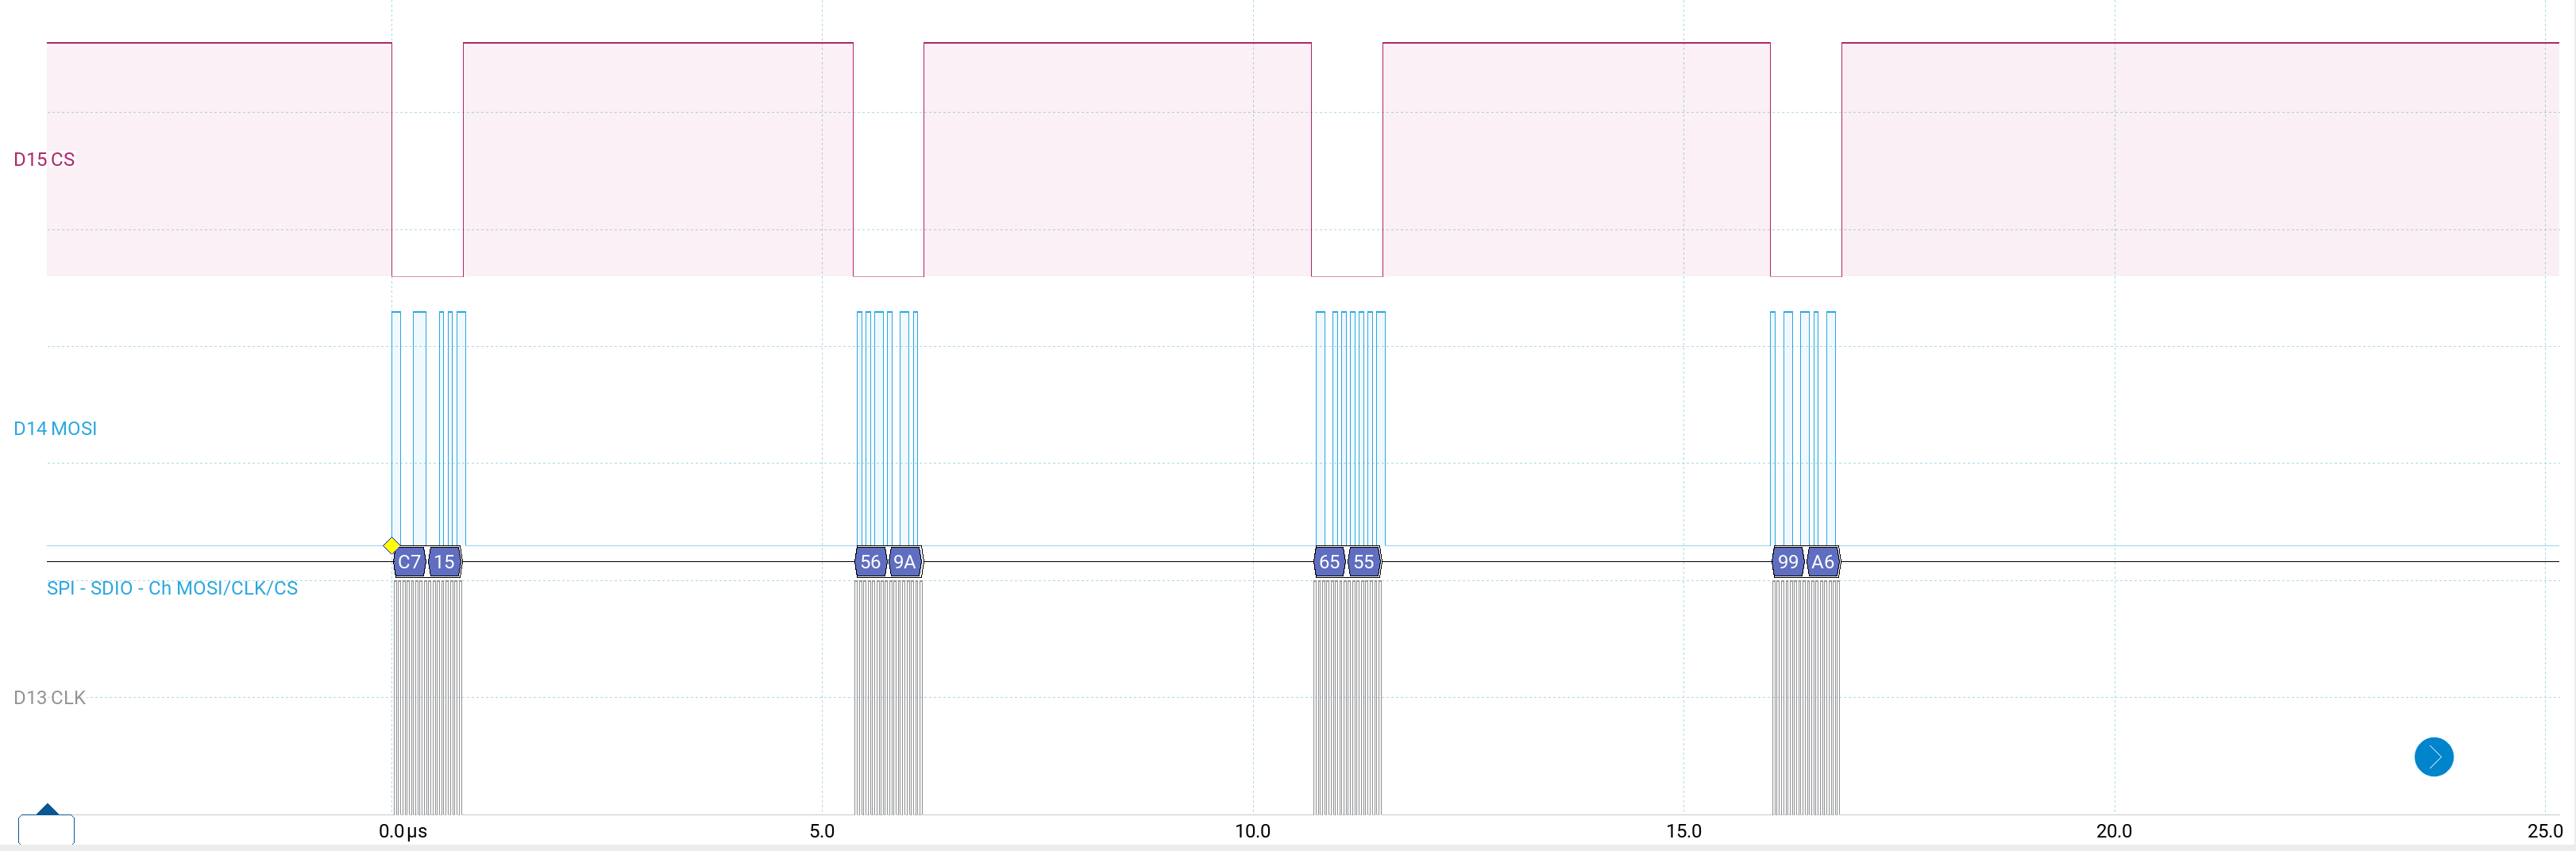
\includegraphics[width=1\linewidth]{Figures/Chap4/FPGA/Test_FPGA_noBuff_signal.png}
    \caption{Ausgegebene Daten des FPGA auf die SPI in Szenario 1 Nutzdatenbyte (16 Bit)}
    \label{fig:ResultatFPGANoBuff}
\end{figure}

Abbildung \ref{fig:ResultatFPGANoBuff} zeigt nur den ersten Teil der ganzen Übertragung. Das ganze übertragene Telegramm ist in Abbildung \ref{fig:ResultatFPGANoBuffFull} zu sehen. Aufgrund der Länge können die Daten nicht angezeigt werden, ohne hinein zu zoomen.
Es sind 32 Übertragungen an 16 Bit zu sehen, was 32 Nutzdatenbytes entsprechen. In der Tabelle \ref{tab:packet_data} sind die aus \textit{Picoscope 7} exportierten Daten aufgelistet, welche zur Abbildung \ref{fig:ResultatFPGANoBuffFull} gehören.

\begin{figure}[H]
    \centering
    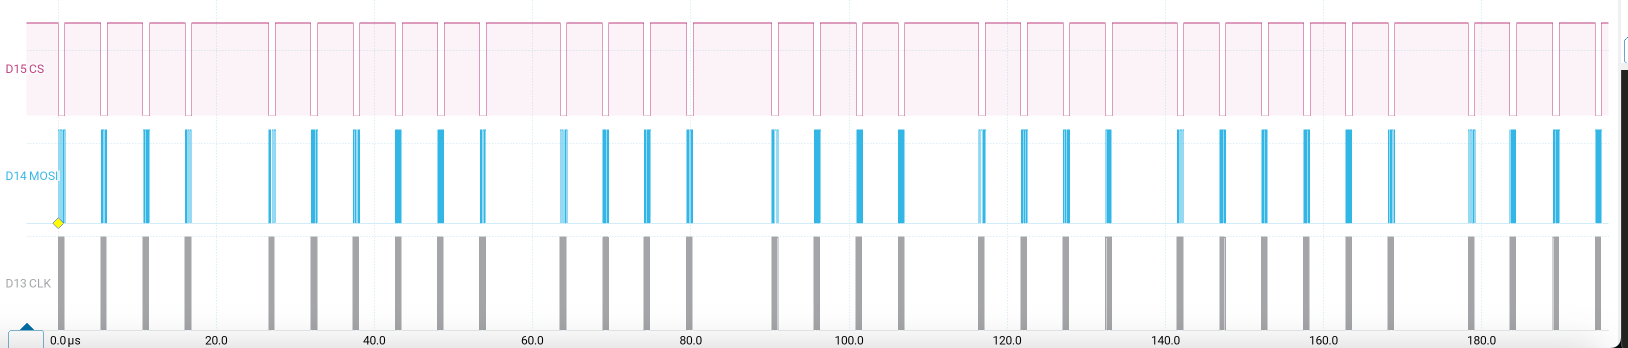
\includegraphics[width=1\linewidth]{Figures/Chap4/FPGA/Test_FPGA_noBuff_signal_full.png}
    \caption{Ausgegebenes ganzes Telegramm des FPGA auf die SPI in Szenario 1 Nutzdatenbyte (16 Bit)}
    \label{fig:ResultatFPGANoBuffFull}
\end{figure}

\begin{table}[h!]
    \centering
    \begin{tabular}{cl||cl||cl||cl}
        \toprule
        \textbf{Packet} & \textbf{Data} & \textbf{Packet} & \textbf{Data} & \textbf{Packet} & \textbf{Data} & \textbf{Packet} & \textbf{Data} \\ 
        \midrule
        1  & C7 15 & 9  & AA AA & 17 & 55 55 & 25 & A9 96 \\
        2  & 56 9A & 10 & 6A 66 & 18 & AA AA & 26 & AA AA \\
        3  & 65 55 & 11 & C7 15 & 19 & C7 15 & 27 & AA AA \\
        4  & 99 A6 & 12 & 55 95 & 20 & 56 99 & 28 & A5 69 \\
        5  & A8 E3 & 13 & 69 55 & 21 & 5A 55 & 29 & C7 15 \\
        6  & 55 65 & 14 & A9 AA & 22 & 6A AA & 30 & 96 56 \\
        7  & 9A 65 & 15 & A8 E3 & 23 & A8 E3 & 31 & 56 55 \\
        8  & AA AA & 16 & 55 55 & 24 & 55 65 & 32 & 6A A9 \\
        \bottomrule
    \end{tabular}
    \caption{Daten 16-Bit Übertragung}
    \label{tab:packet_data}
\end{table}

Die Abbildungen und die Tabelle entsprechen einem übertragenen Telegramm. Im Test fanden viel mehr Übertragungen statt. Dabei konnten keine, zu den gezeigten Daten, abweichenden Werte festgestellt werden.

\subsection{Test mit 64-Bit-Puffer Implementierung}
\label{sub:ResultatFPGABuff}
Im zweiten Testszenario konnten je nach Zeit, zwischen den gesendeten Telegramme, verschiedene Resultate beobachtet werden. In Abbildung \ref{fig:ResultatFPGABuff} ist die Übertragung eines ganzen Telegrammes zu sehen. In diesem Fall handelt es sich um die gleiche Anzahl übertragener Bit wie in Kapitel \ref{sub:ResultatFPGAnoBuff}, jedoch wurden diese jeweils in acht 64-Bit Pakete übertragen.

\begin{figure}[H]
    \centering
    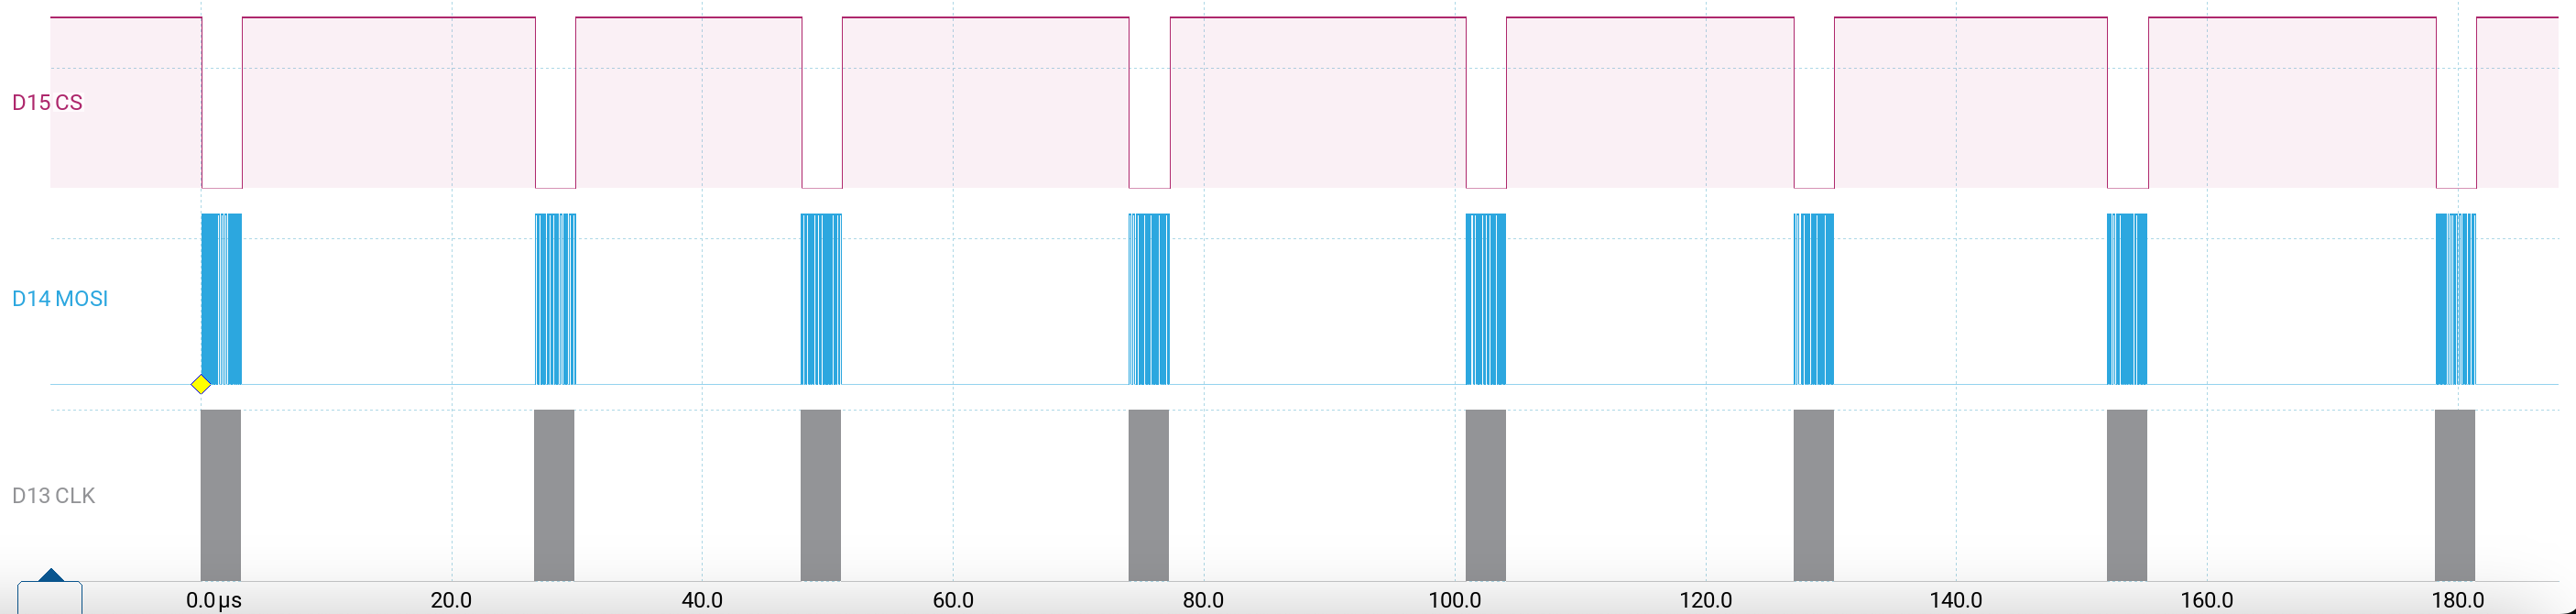
\includegraphics[width=1\linewidth]{Figures/Chap4/FPGA/Test_FPGA_Buff_signal.png}
    \caption{Ausgegebene Daten des FPGA auf die SPI in Szenario Puffer (64 Bit)}
    \label{fig:ResultatFPGABuff}
\end{figure}

Die übertragenen Daten, wenn alle 100 ms ein Telegramm ausgegeben wurde, sind in der Tabelle \ref{tab:packet_data_2cols} zu sehen. 

\begin{table}[h!]
    \centering
    \begin{tabular}{c||l}
        \toprule
        \textbf{Packet} & \textbf{Data} \\ 
        \midrule
        1 & C7 15 56 9A 65 55 99 A6 \\
        2 & A8 E3 55 65 9A 65 AA AA \\
        3 & AA AA 6A 66 C7 15 55 95 \\
        4 & 69 55 A9 AA A8 E3 55 55 \\
        5 & 55 55 AA AA C7 15 56 99 \\
        6 & 5A 55 6A AA A8 E3 55 65 \\
        7 & A9 96 AA AA AA AA A5 69 \\
        8 & C7 15 96 56 56 55 6A A9 \\
        \bottomrule
    \end{tabular}
    \caption{Übertragene Daten auf SPI; 100 ms; 64 Bit}
    \label{tab:packet_data_2cols}
\end{table}

Es ist zu sehen dass zwischen den erhaltenen Daten und den erwarteten Daten, welche in der Tabelle \ref{tab:frame_data} in der Spalte \textit{Data} abgebildet sind, keine Abweichungen festzustellen sind.

Wenn jede ms eine Übertragung statt findet, so sind zu den in der Tabelle \ref{tab:frame_data} sehende Anordnung der Daten, Abweichungen festzustellen. Grundsätzlich werden die gleichen Daten übermittelt aber oftmals an einer anderen Stelle und teilweise wurden nicht alle Pakete übertragen. Selten werden auch falsche Daten übermittelt.

In der Tabelle \ref{tab:data_table} sind die Daten eines Telegramms zu sehen, welches fehlerhaft war. Beim Achten Packet ist zu sehen dass anstatt \textit{"'C7 15 96 56 56 55 6A A9"'} die falschen Daten \textit{"'00 0F 8E 2B 2C AC AC AA"'} übermittelt wurden.

\begin{table}[h!]
    \centering
    \begin{tabular}{c||l}
        \toprule
        \textbf{Packet} & \textbf{Data} \\ 
        \midrule
        1 & C7 15 56 9A 65 55 99 A6 \\
        2 & A8 E3 55 65 9A 65 AA AA \\
        3 & AA AA 6A 66 C7 15 55 95 \\
        4 & 69 55 A9 AA A8 E3 55 55 \\
        5 & 55 55 AA AA C7 15 56 99 \\
        6 & 5A 55 6A AA A8 E3 55 65 \\
        7 & A9 96 AA AA AA AA A5 69 \\
        8 & 00 0F 8E 2B 2C AC AC AA \\
        \bottomrule
    \end{tabular}
    \caption{Übertragene Daten auf SPI; 1 ms; 64 Bit}
    \label{tab:data_table}
\end{table}




%---------------------------------------------------------------------------------
% SECTION 2
%---------------------------------------------------------------------------------

\section{Firmware ESP32}
\label{sec:ResultatESP32}
%\textcolor{red}{Erstes Resultat des ESP: SPI ist nicht genügend schnell, um die Packete des FPGA entgegen zu nehmen}

Der Test der Firmware des ESP32-S3 wurde gemäss Kapitel \ref{sub:ESPSPIundFSMTest} durchgeführt. Als Erstes wurde das kurze Telegramm getestet und der Pin 21 wurde nicht auf Ground verbunden. Durch Drücken der Boot-Taste auf dem SPI-Master wird das Senden getriggert. In Abbildung \ref{fig:ResultatBLEKurz} ist die Anzeige in der Applikation \textit{Bluetility} gezeigt und Einfärbungen gemacht, welche Teile zu den Daten gehören.

\begin{figure}[H]
    \centering
    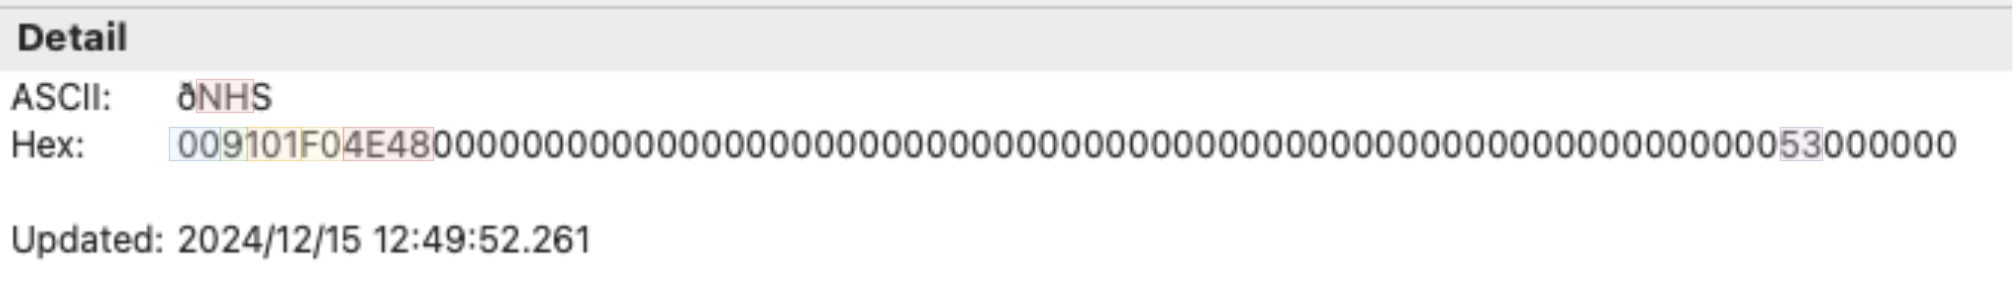
\includegraphics[width=0.9\linewidth]{Figures/Chap4/ESP32/Resultat_BLE_kurz.png}
    \caption{Resultat Bluetility kurzes Telegram}
    \label{fig:ResultatBLEKurz}
\end{figure}

Die Daten werden in der Struktur aus Kapitel \ref{subsub:DataTelegramm} übertragen und sind wie folgt:

\begin{itemize}[noitemsep]
    \item metadata: 0x00 --> Keine Fehler im Telegramm
    \item data\_m: 0x9101 --> FCode: 9; Adresse: 0x101
    \item check\_m: 0xF0 --> Dummy Check Data
    \item data\_s: 0x4E48 --> ASCII für "'NH"'
    \item check\_s: 0x53 --> Dummy Check Data
\end{itemize}

%Die Aufzeichnung der Reaktionszeit für das kurze Telegramm mit dem Oszilloskop ist in Abbildung \ref{fig:ReakKurz} zu sehen. Die orange Linie ist dabei die \textit{Chip Select} Leitung und die blaue Linie die \textit{Handshakeleitung}. 

\begin{figure}[H]
    \centering
    % Erstes Bild
    \begin{subfigure}[b]{0.45\textwidth}
        \centering
        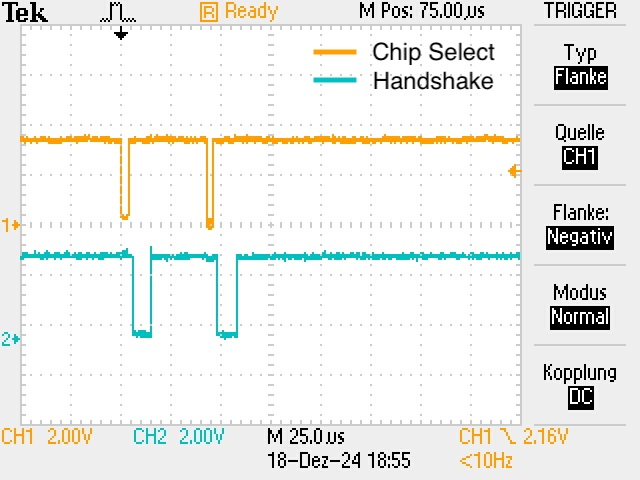
\includegraphics[width=\linewidth]{Figures/Chap4/ESP32/Gesammte Transaktion Kurz.JPG} 
        \caption{Insgesamt 2 Transaktionen}
        \label{fig:GesTransKurz}
    \end{subfigure}
    \hfill 
    %Zweites Bild
    \begin{subfigure}[b]{0.45\textwidth}
        \centering
        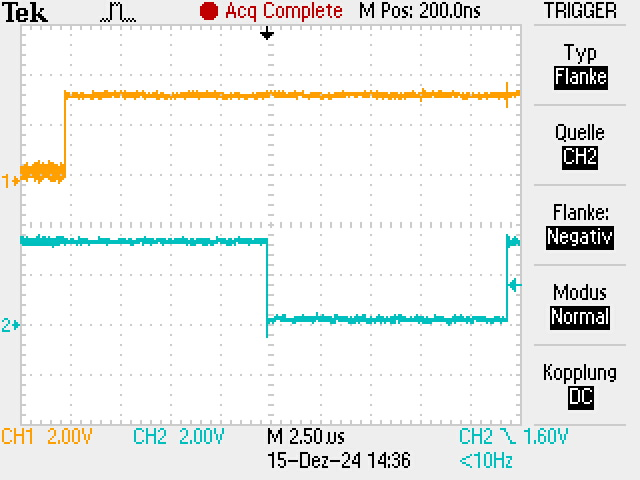
\includegraphics[width=\linewidth]{Figures/Chap4/ESP32/Reaktionszeit Kurz.JPG} 
        \caption{Vergrösserung im Zeitbereich der Reaktionszeit bei kurzem Telegramm}
        \label{fig:ReakKurz}
    \end{subfigure}
    \caption{Resultat der Reaktionszeit kurzes Telegramm gemessen mit dem Oszilloskop}
    \label{fig:ResultatOsziReaktionKurz} 
\end{figure}

In Abbildung \ref{fig:GesTransKurz} ist ersichtlich, dass das vollständige Telegramm nach 2 Transaktionen abgeschlossen ist. Dies kann anhand der negativen Pulse der Chip-Select Leitung gezählt werden.
In Abbildung \ref{fig:ReakKurz} sind die Zeiten gut zu sehen. Die in Kapitel \ref{sub:ESPSPIundFSMTest} definierten Zeiten lauten:
\begin{itemize}
    \item Reaktionszeit: 2 $\mu$s
    \item BTR-Zeit: 12 $\mu$s
\end{itemize}


Als Zweites wurde das lange Telegramm getestet. In Abbildung \ref{fig:ResultatBLELang} ist die Anzeige in der Applikation \textit{Bluetility} gezeigt und Einfärbungen gemacht, welche Teile zu den Daten gehören.

\begin{figure}[H]
    \centering
    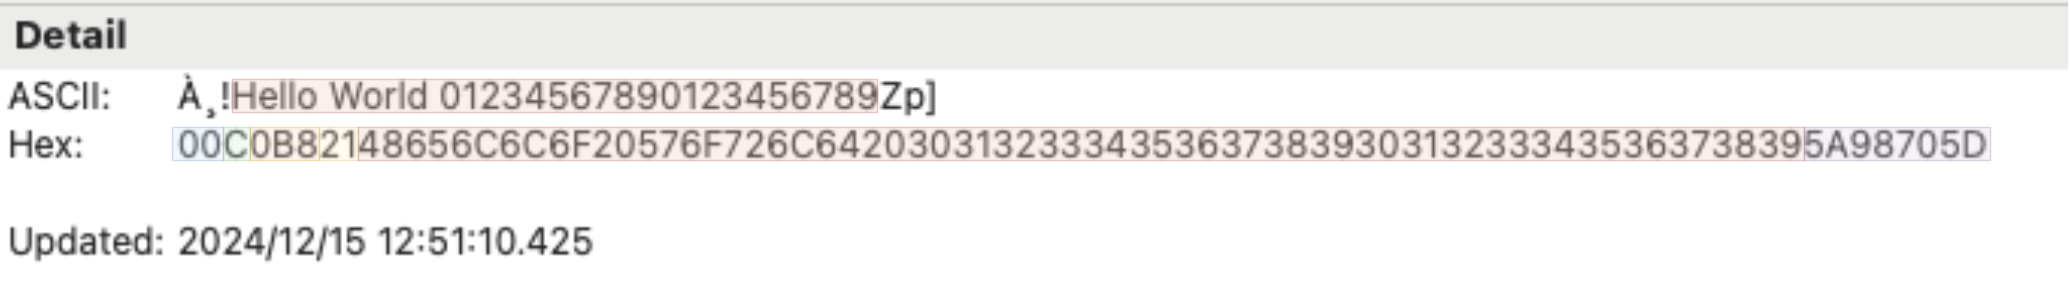
\includegraphics[width=0.9\linewidth]{Figures/Chap4/ESP32/Resultat_BLE_lang.png}
    \caption{Resultat Bluetility langes Telegram}
    \label{fig:ResultatBLELang}
\end{figure}

Die Daten werden wieder in der Struktur aus Kapitel \ref{subsub:DataTelegramm} übertragen und sind wie folgt:

\begin{itemize}[noitemsep]
    \item metadata: 0x00 --> Keine Fehler im Telegramm
    \item data\_m: 0xC0B8 --> FCode: 0xC (12); Adresse: 0x0B8
    \item check\_m: 0x21 --> Dummy Check Data
    \item data\_s: \textit{siehe Bild} --> ASCII für "'Hello World 01234567890123456789"'
    \item check\_s: 0x5A'98'70'5D --> Dummy Check Data der Reihe nach 0x[0]'[1]'[2]'[3]
\end{itemize}

\begin{figure}[H]
    \centering
    % Erstes Bild
    \begin{subfigure}[b]{0.45\textwidth}
        \centering
        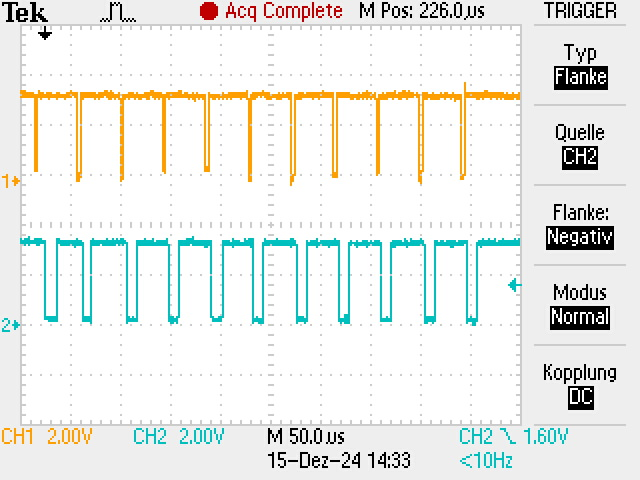
\includegraphics[width=\linewidth]{Figures/Chap4/ESP32/Gesammte Transaktion Lang.JPG} 
        \caption{Insgesamt 11 Transaktionen}
        \label{fig:GesTransLang}
    \end{subfigure}
    \hfill 
    %Zweites Bild
    \begin{subfigure}[b]{0.45\textwidth}
        \centering
        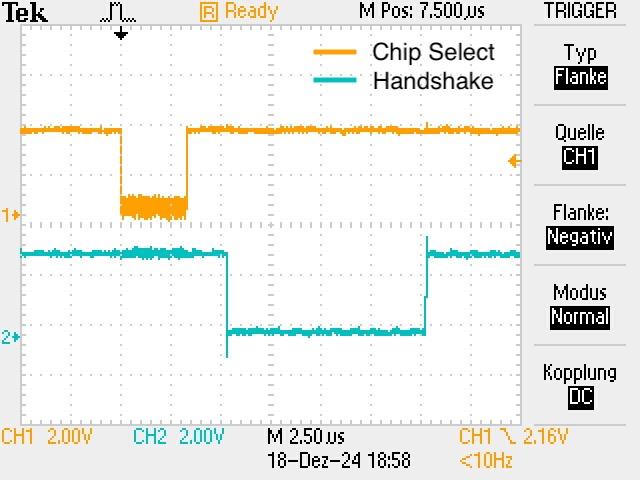
\includegraphics[width=\linewidth]{Figures/Chap4/ESP32/Reaktionszeit Lang.JPG} 
        \caption{Vergrösserung im Zeitbereich der Reaktionszeit bei langem Telegramm}
        \label{fig:ReakLang}
    \end{subfigure}
    \caption{Resultat der Reaktionszeit langem Telegramm gemessen mit dem Oszilloskop}
    \label{fig:ResultatOsziReaktionLang} 
\end{figure}

In Abbildung \ref{fig:GesTransLang} ist ersichtlich, dass das vollständige Telegramm nach 11 Transaktionen abgeschlossen ist. Dies kann anhand der negativen Pulse der Chip-Select Leitung gezählt werden.
In Abbildung \ref{fig:ReakLang} sind die Zeiten zu sehen. Die in Kapitel \ref{sub:ESPSPIundFSMTest} definierten Zeiten lauten:
\begin{itemize}
    \item Reaktionszeit: 2 $\mu$s
    \item BTR-Zeit: 12 $\mu$s
\end{itemize}


%\href{https://docs.espressif.com/projects/esp-idf/en/stable/esp32s3/api-reference/peripherals/spi_slave.html#transaction-interval}{ESP-IDF SPI Slave Transaction Interval}


\section{Übertragungstest SPI}
\label{sec:ResultatÜbertragungSPI}
Um die Übertragung der Daten vom FPGA zum ESP32-S3 zu überprüfen, wurde ein Test gemäss Kapitel \ref{subsec:VerbindugstestESP32FPGA} durchgeführt.

Für das Triggerintervall von 3 Sekunden ist folgendes Resultat entstanden. Auf der \textit{Bluetify}-Applikation sind die folgenden Notifikationen empfangen worden:

\begin{table}[H]
    \centering
    \begin{tabular}{r||c|c|c|c}
        \hline
        Frame Nr & 1 & 2 & 3 & 4\\ \hline
        meta data & 0x00 & 0x00 & 0x00 & 0x01\\ \hline
        data\_m & 0x1B40 & 0x0860 & 0x1A30 & 0x9110\\ \hline
        check\_m & 0xAD & 0xEF & 0x7F & 0x7E\\ \hline
        data\_s & 0x04B4FFFF & 0x0000 & 0x04E9FFFF & -\\ \hline
        check\_s & 0x75 & 0xFF & 0xC6 & -\\ \hline
    \end{tabular}
    \caption{Empfangene Telegramme bei Triggerinterval 3 s}
    \label{tab:EmpfTeleg3sTrigg}
\end{table}

Mit dem Picoscope wurde das Signal im digitalen Bereich aufgezeignet, sodass die Reaktionszeit und die Back-to-Receive-Zeit bestimmt werden konnten. 

\begin{figure}
    \centering
    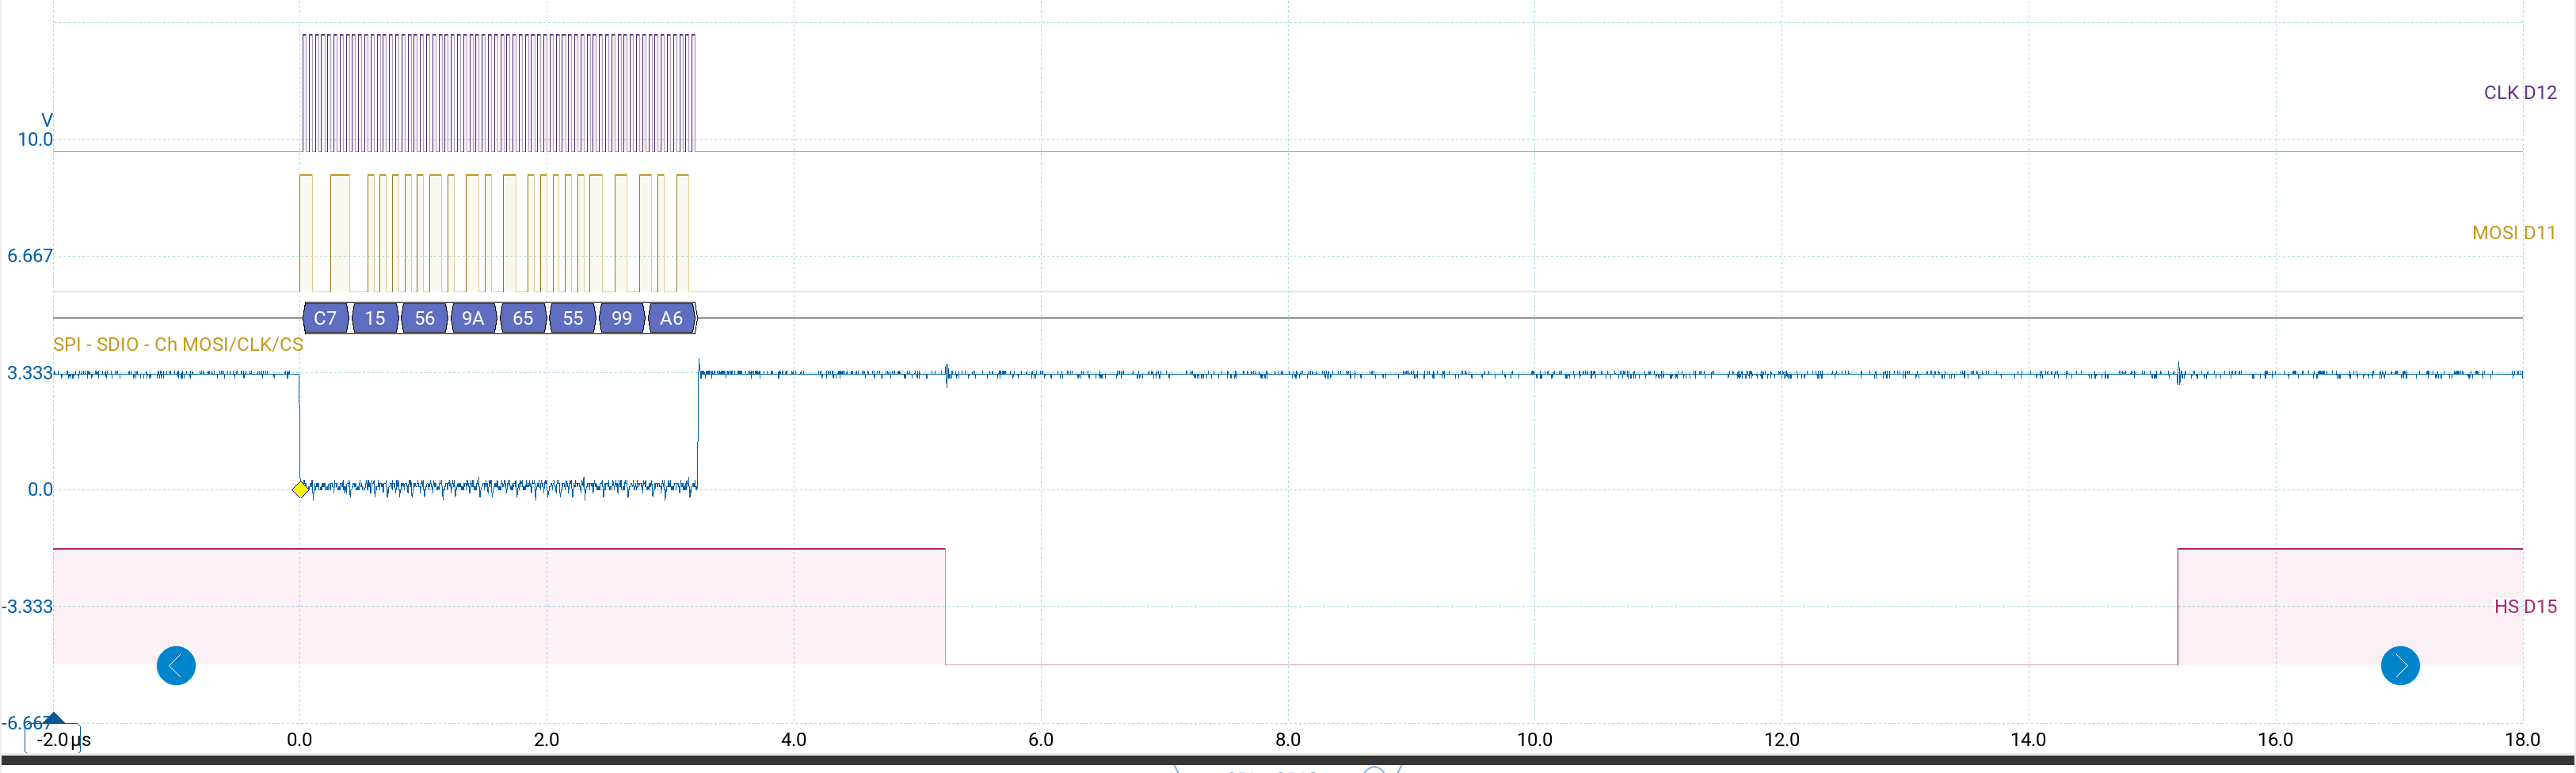
\includegraphics[width=\linewidth]{Figures/Chap4/Verbindungstest_SPI/VerbindungstestZeiten.png}
    \caption{Erstes 64-Bit Packet}
    \label{fig:VerbindungstestZeiten}
\end{figure}

In Abbildung \ref{fig:VerbindungstestZeiten} ist die Messung mit dem Picoscope zu sehen. Die oberste Kurve ist die Clock-Leitung, darunter folgt die MOSI-Leitung, darunter in Blau dargestellt die Chip-Select-Leitung und zu unterst die Handshake-Leitung.

Die in Kapitel \ref{sub:ESPSPIundFSMTest} definierten Zeiten lauten:
\begin{itemize}
    \item Reaktionszeit: 2 $\mu$s
    \item BTR-Zeit: 12 $\mu$s
\end{itemize}


\section{Stresstest FPGA und ESP32}
\label{sec:ResStresstest}

Der Stresstest wurde, wie in Kapitel \ref{sub:MethStesstest} beschrieben, durchgeführt.

Das Resultat für das Triggerintervall von 50 ms ist in Abbildung \ref{fig:Stress50} zu sehen. Die gemessenen Telegramme für die Erstellung der Grafik ist in Anhang \ref{app:File63_50ms} zu finden. Die vier häufigsten Telegramme sind die erwarteten Telegramme aus Tabelle \ref{tab:frame_data}.

\begin{figure}[H]
    \centering
    \begin{minipage}{0.29 \textwidth}
        \begin{tabular}{c||c}
            \toprule
            \textbf{Anzahl} & \textbf{Frame Nr} \\ 
            \midrule
            469 &  1\\
            469 & 2 \\
            469 & 3 \\
            468 & 4 \\
            \bottomrule
        \end{tabular}
    \end{minipage}
    \hfill
    \begin{minipage}{0.7 \textwidth}
        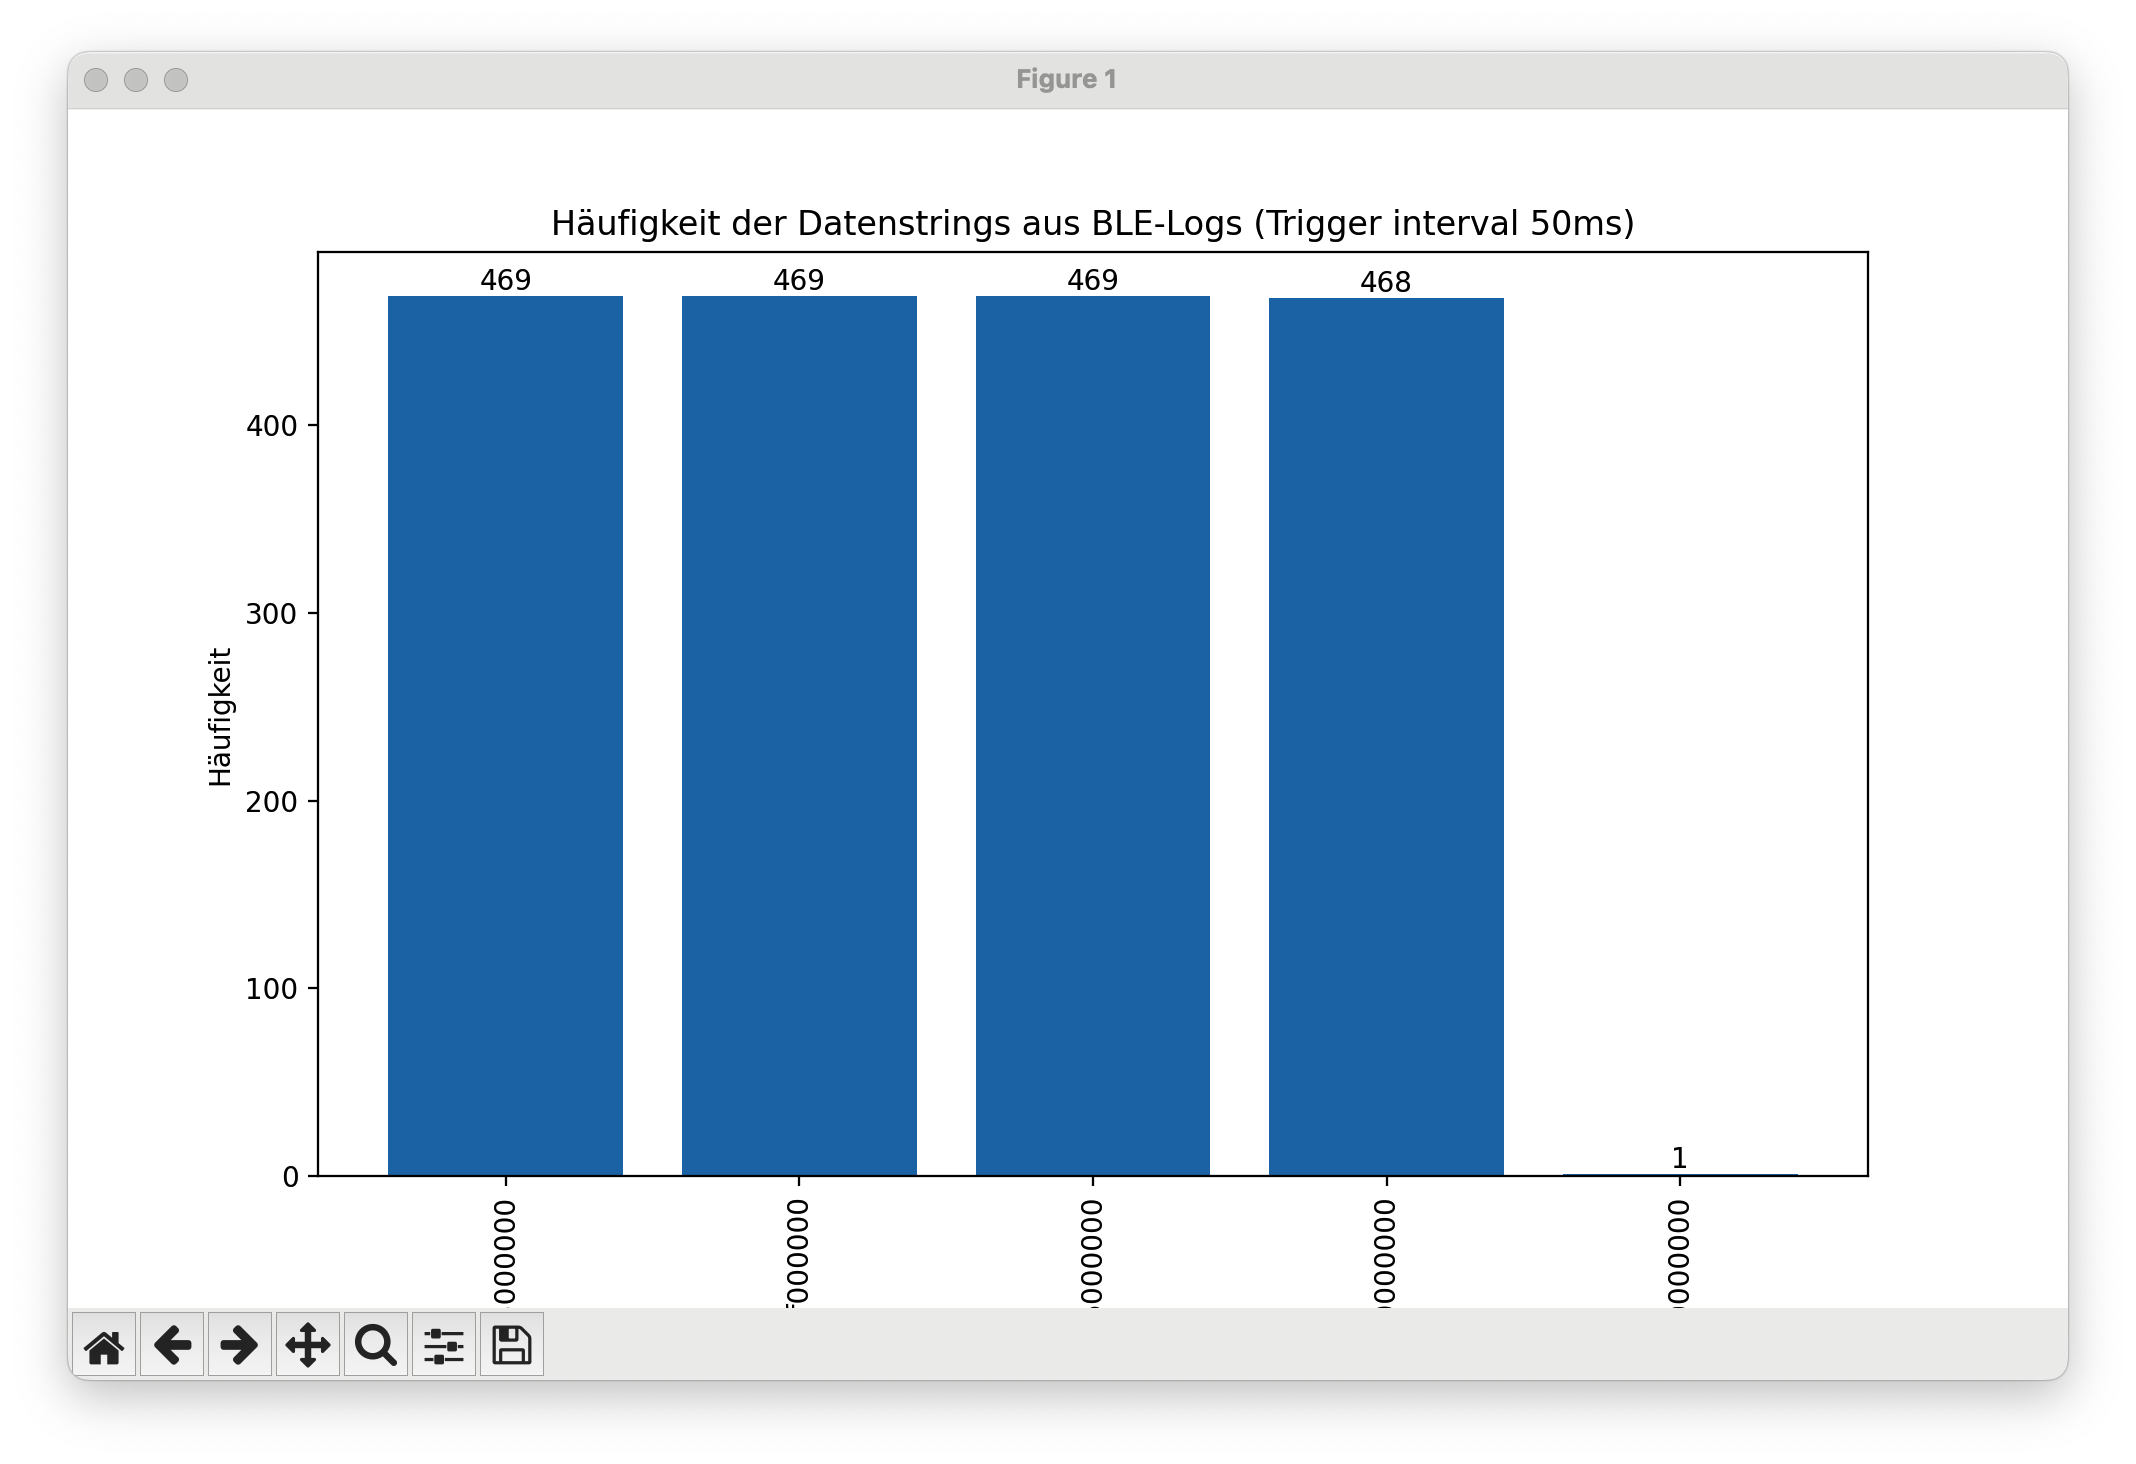
\includegraphics[width = \linewidth]{Figures/Chap4/Stesstest/Stress_50.png}
    \caption{Stresstest Triggerintervall 50 ms}
    \label{fig:Stress50}
    \end{minipage}
\end{figure}


Das Resultat für das Triggerintervall von 25 ms ist in Abbildung \ref{fig:Stress25} zu sehen. Die gemessenen Telegramme für die Erstellung der Grafik ist in Anhang \ref{app:File64_25ms} zu finden. Die vier häufigsten Telegramme sind die erwarteten Telegramme aus Tabelle \ref{tab:frame_data}.

\begin{figure}[H]
    \centering
    \begin{minipage}{0.29 \textwidth}
        \begin{tabular}{c||c}
            \toprule
            \textbf{Anzahl} & \textbf{Frame Nr} \\ 
            \midrule
            932 & 1\\
            932 & 2\\
            929 & 3\\
            925 & 4\\
            \bottomrule
        \end{tabular}
    \end{minipage}
    \hfill
    \begin{minipage}{0.7 \textwidth}
        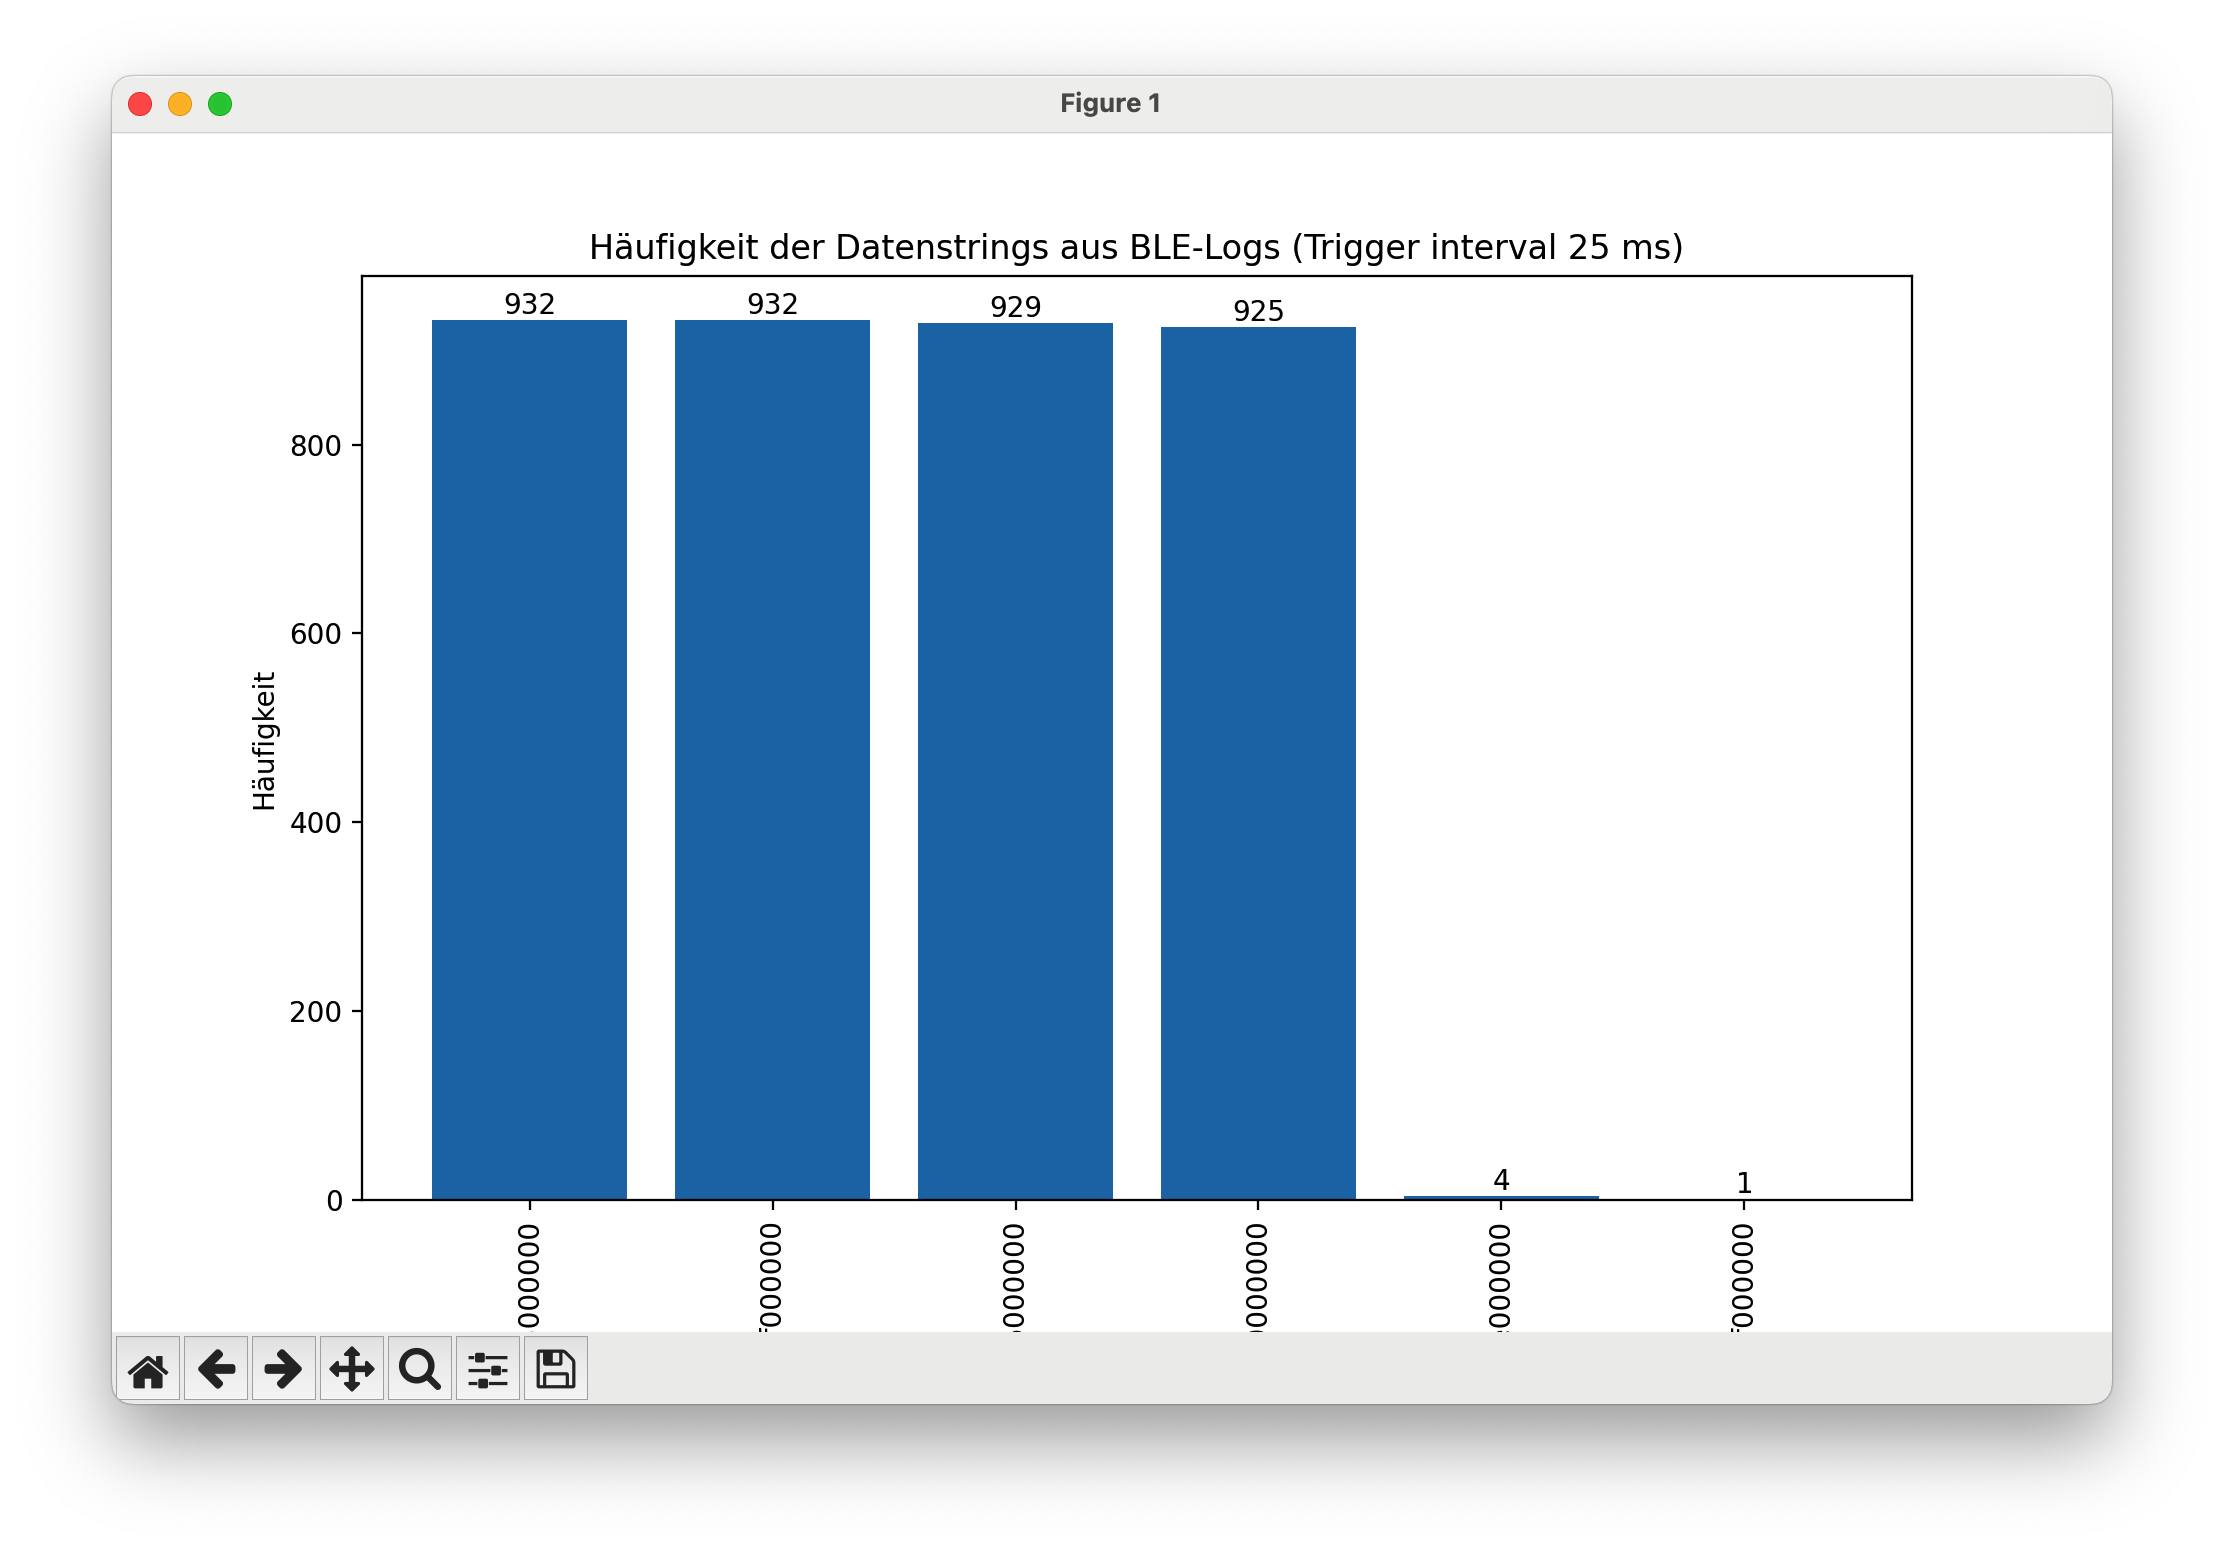
\includegraphics[width=\linewidth]{Figures/Chap4/Stesstest/Stress_25.png}
    \caption{Stresstest Triggerintervall 25 ms}
    \label{fig:Stress25}
    \end{minipage}
\end{figure}

Das Resultat für das Triggerintervall von 12.5 ms ist in Abbildung \ref{fig:Stress12_5} zu sehen. Die gemessenen Telegramme für die Erstellung der Grafik ist in Anhang \ref{app:File65_12_5ms} zu finden. Die vier häufigsten Telegramme sind die erwarteten Telegramme aus Tabelle \ref{tab:frame_data}.

\begin{figure}[H]
    \centering
    \begin{minipage}{0.29 \textwidth}
        \begin{tabular}{c||c}
            \toprule
            \textbf{Anzahl} & \textbf{Frame Nr} \\ 
            \midrule
            1600 & 1\\
            1553 & 2\\
            1468 & 4\\
            1340 & 3\\
            \bottomrule
        \end{tabular}
    \end{minipage}
    \hfill
    \begin{minipage}{0.7 \textwidth}
        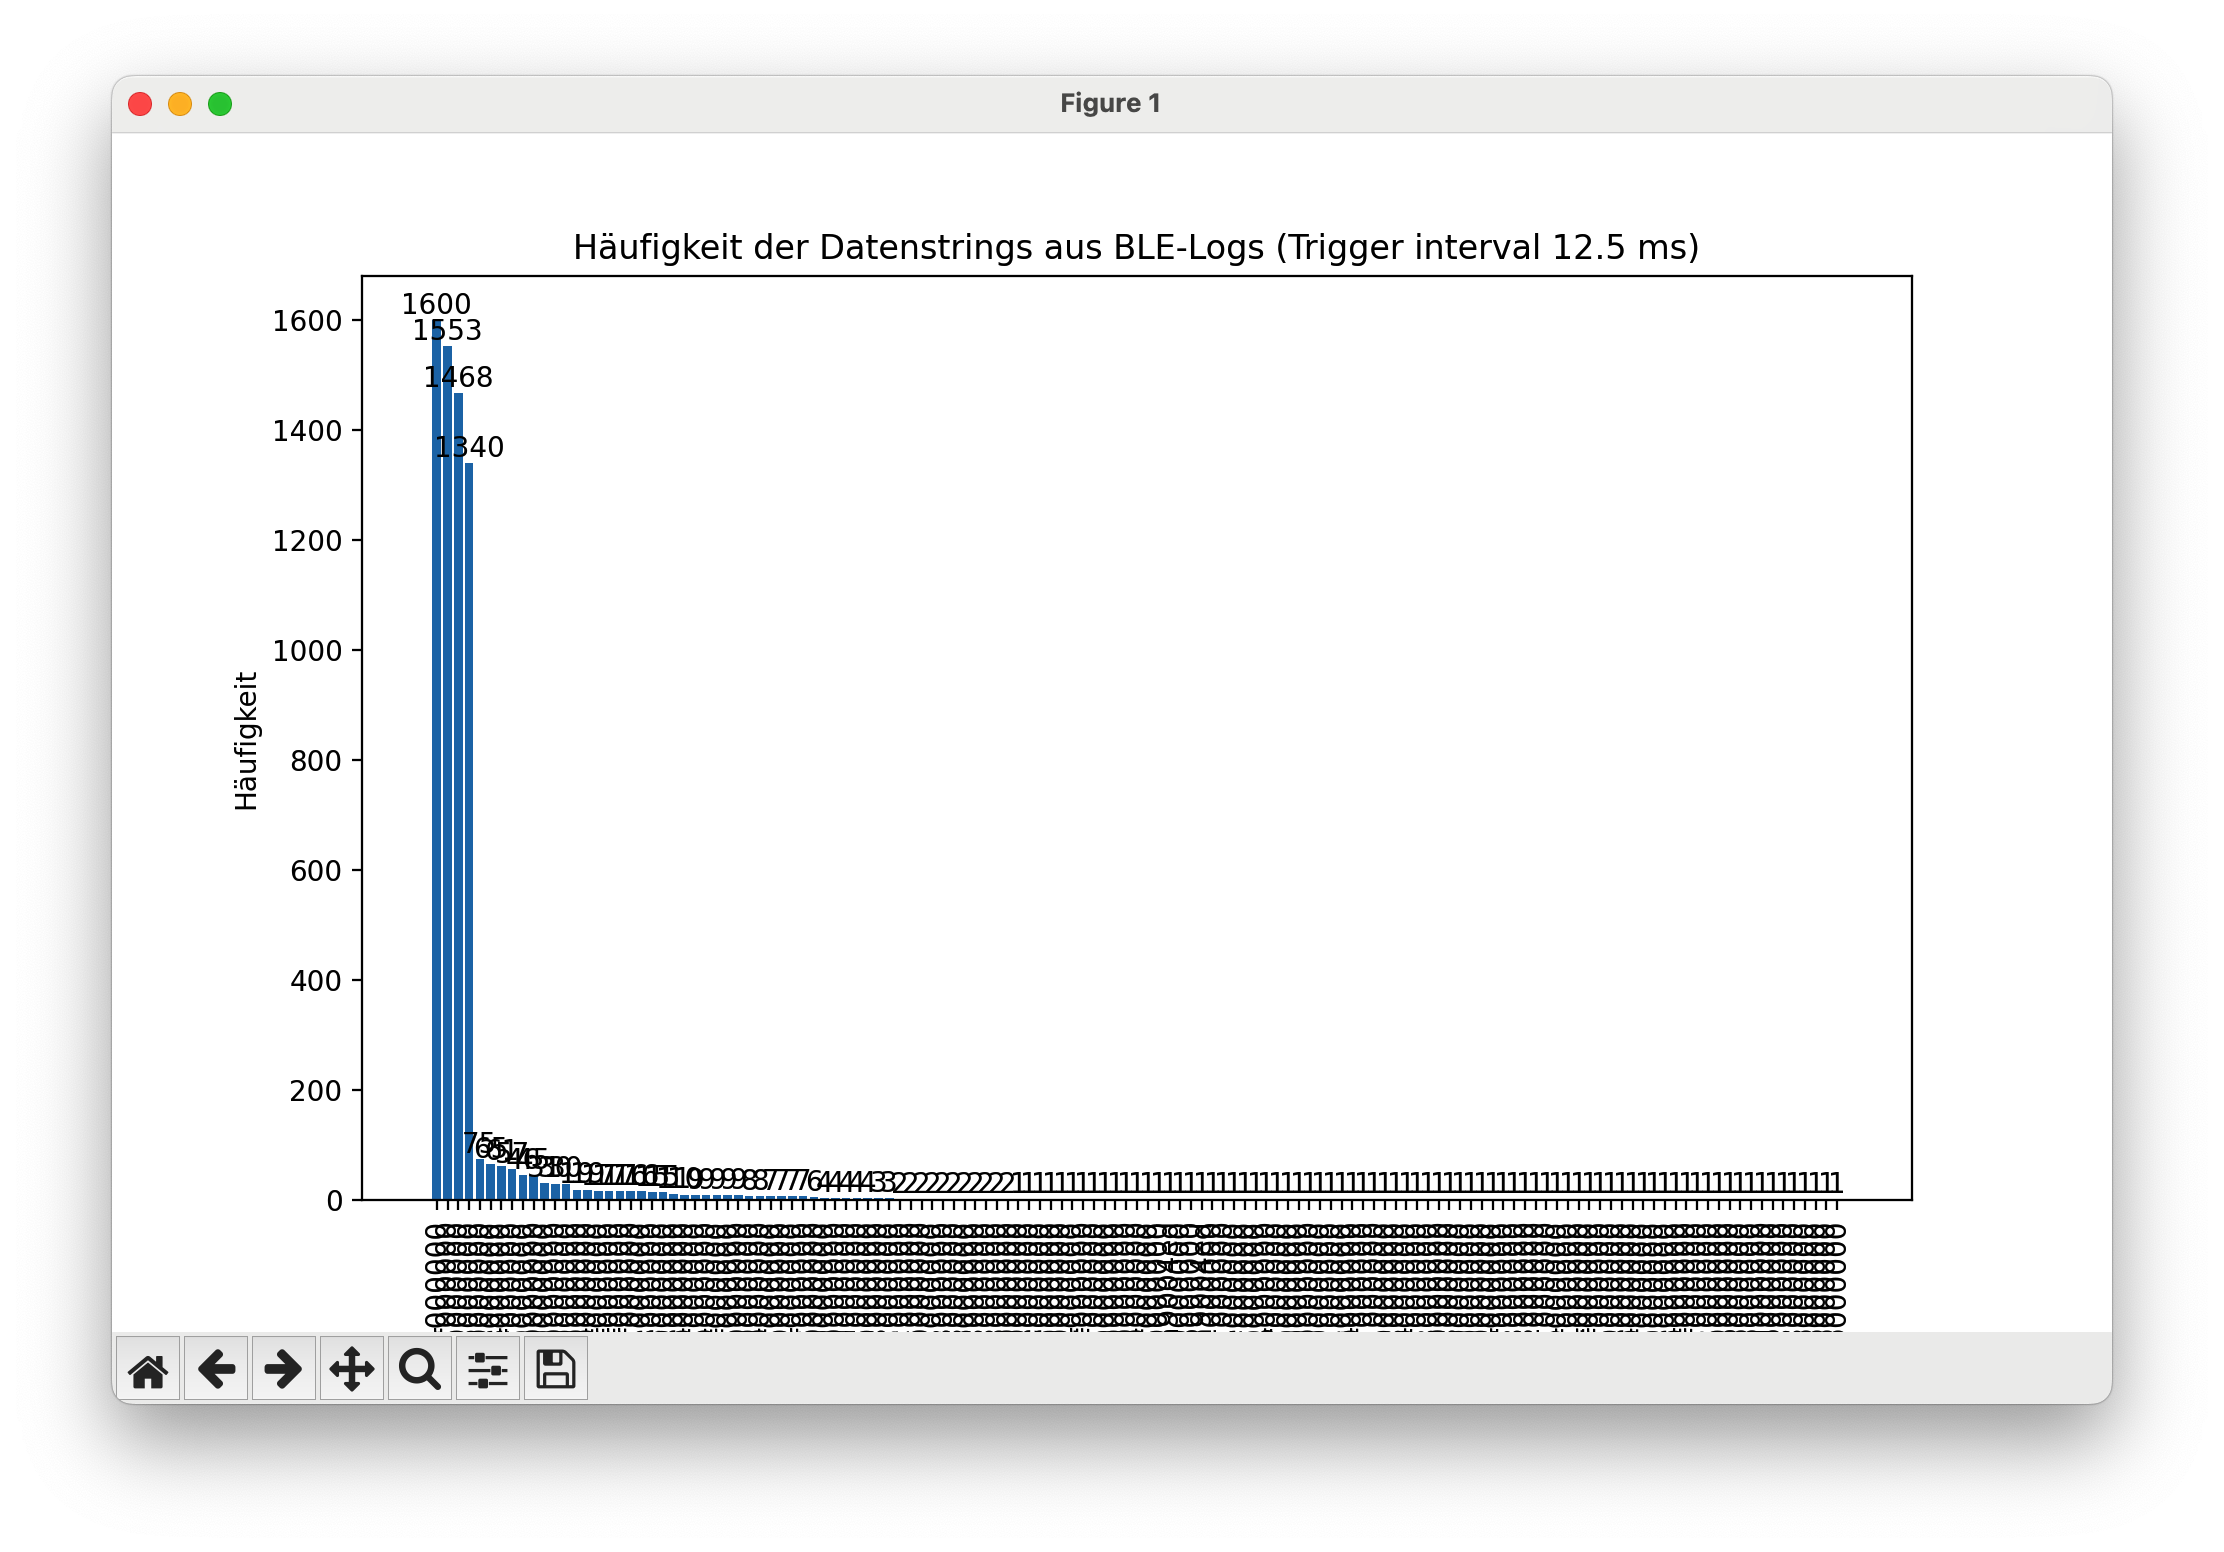
\includegraphics[width=\linewidth]{Figures/Chap4/Stesstest/Stress_12_5.png}
    \caption{Stresstest Triggerintervall 12.5 ms}
    \label{fig:Stress12_5}
    \end{minipage}
\end{figure}

\newpage

Das Resultat für das Triggerintervall von 1 ms ist in Abbildung \ref{fig:Stress1} zu sehen. Die gemessenen Telegramme für die Erstellung der Grafik ist in Anhang \ref{app:File66_1ms} zu finden. Die vier häufigsten Telegramme sind die erwarteten Telegramme aus Tabelle \ref{tab:frame_data}.

\begin{figure}[H]
    \centering
    \begin{minipage}{0.29 \textwidth}
        \begin{tabular}{c||c}
            \toprule
            \textbf{Anzahl} & \textbf{Frame Nr} \\ 
            \midrule
            6191 & 4\\
            891 & 2 \\
            720 & 1 \\
            507 & 3 \\
            \bottomrule
        \end{tabular}
    \end{minipage}
    \hfill
    \begin{minipage}{0.7 \textwidth}
        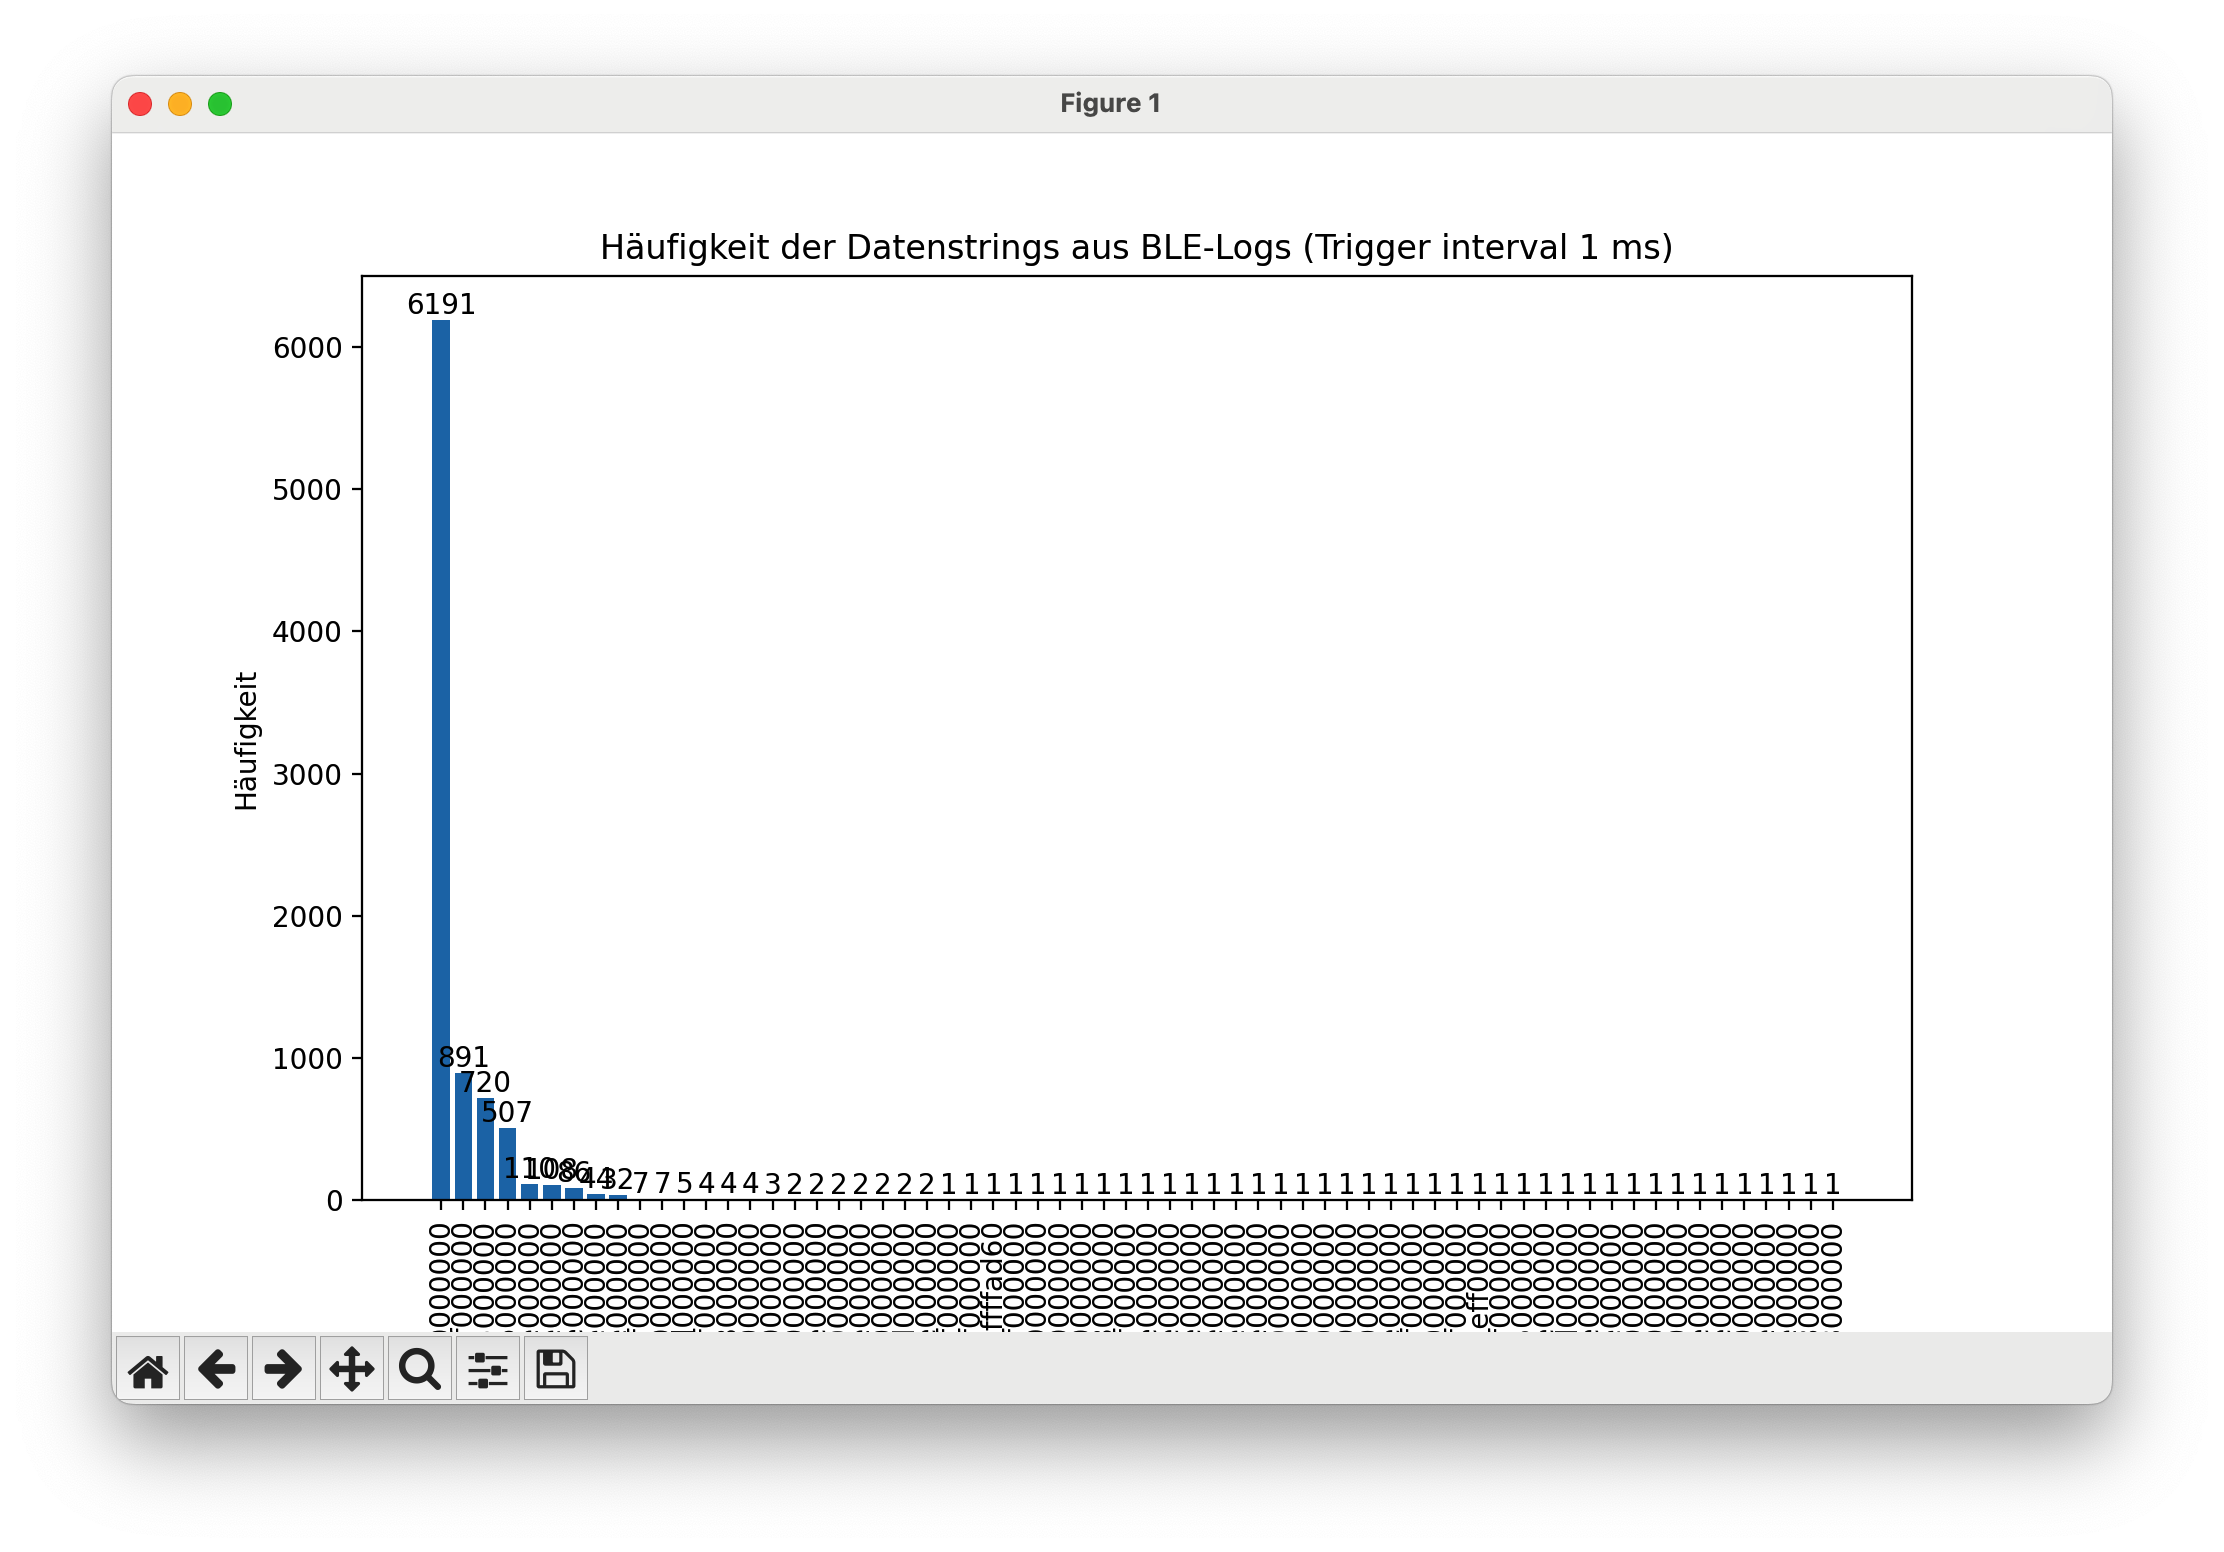
\includegraphics[width=\linewidth]{Figures/Chap4/Stesstest/Stress_1.png}
    \caption{Stresstest Triggerintervall 1 ms}
    \label{fig:Stress1}
    \end{minipage}
\end{figure}

Zusammenfassend wurden vier Messungen von ungefähr 20-30 Sekunden durchgeführt und die resultierenden Plots eingefügt.

\section{Hardware Design}
\label{sec:ResultatHardware}
Im Rahmen dieser Arbeit wurde ein Schema für den MVB-Sniffer in der Software Altium entworfen. Es wurde darauf geachtet, die zentralen Rollen der Komponenten, übersichtlich zu gestalten, dass ihre Interaktionen und Funktionalitäten nachvollziehbar sind. Diese wurden ebenfalls detailliert im Kapitel \ref{sec:Hardware Design} erläutert. Das entwickelte Schema erfüllt die aktuellen Anforderungen von den zusammengeführten Evaluationsboards, wurde kompakter gestaltet durch Reduzierung von nicht benötigter Komponenten und Verbindungen und bietet eine Basis für zukünftige Erweiterungen des Sniffers. 

Das Schema ist auf 5 Seiten aufgeteilt. Auf der ersten Seite befinden sich die Anschlüsse an den MVB, die Verbindung zu dem RS485-Transreceiver und alle In- und Outputs von den Banken. Die zweite Seite wurde für die DC/DC-Wandler verwendet, die Interaktionen die über Taster und einen Schalter mit dem FPGA gemach twerden können, sowie die JTAG Schnittstelle und der Oszillator für den FPGA. Auf der dritten Seite sind die Spannungsversorgungen und Ground Anbindungen. Seite 4 zeigt den ESP32, dessen USB Schnittstellen, den 3 Drucktastern für Interaktionen mit dem ESP32, die USB-UART-Brücke und die Transistoren Schaltung um den ESP32 in die 3 Modi zu versetzen. Auf der Seite 5 ist der Darlington-Array für die Ansteuerung der Zustands LED und die Pinleiste, sowie der Spannungsteiler für die zukünftige Akkumessung. 

Der gesamte Altium Projektordner befindet sich gezippt im Anhang \ref{app:File58}.







% \section{Resultat} % 
% \textcolor{red}{Was ist beim Test herausgekommen. Was hat funktionniert, was nicht?}

